
%\chapter{Project's Objectives and Specification}
 \chapter{Obiective și specificații}
\label{cap:obiective-specificatii}

%Acest capitol conține descrierea detaliată a temei de cercetare propriu-zise, formulată exact, cu obiective clare și specificații, pe 2-3 pagini și eventuale figuri explicative. Titlul nu e neapărat impus și, de asemenea, capitolul poate fi inclus ca subcapitol în Capitolul~\ref{cap:Introducere}, dacă se potrivește.
%
%Reprezintă cca. 5--10\% din lucrare.

Acest capitol prezinta obiectivele lucrarii, motivand deciziile luate in implementarea sistemului, specificatiile sitemului, cerintele functionale si nonfunctionale necesare implementarii sistemului.

%\section{Objectives}
 \section{Obiective}
%
%Obiectivele proiectului sunt lucrurile care se dorește a fi realizate, ca urmare a abordării temei lucrării de licență. În general numărul de obiective este proporțional cu timpul de care dispunem. Exemple generice:
%\begin{enumerate}
%  \item Analiza critică a soluțiilor existente pentru problema abordată și identificarea posibile limitări ale acestora.
%  \item Propunerea unor soluții la (o parte) din problemele identificate. 
%  \item Implementarea soluției și validarea ei
%  \item Identificarea unor teme de dezvoltare și cercetare ulterioare
%  \item \dots
%\end{enumerate}
Elaborarea unor masuri de securitate impotriva anumitor tipuri de atacuri sau dezvoltarea unei logici de filtrare a clientilor serviti de catre aplicatie este posibila si in partea de implementare a serverului, cea ce ar putea oferi si o eventuala crestere in performantele aplicatiei, eliminand astfel posibile interceptari suplimentare si validari ale traficului. Insa o astfel de implementare presupune o arhitectura mult mai complexa pentru partea de server si individual cunostinte avansate despre securitate, posibilele vulnerabilitati la care acesta poate sa fie predispus, precum si modalitati de combatere ale acestora. 

O solutie mult mai simpla la aceasta problema este folosirea unui modul care sa implementeze aceste functionalitati separat. Mare parte din produsele de pe piata, ce indeplinesc aceste caracteristici sunt destul de scumpe si nu ofera foarte multa libertate din punctul de vedera al configurari securitatii dorite de catre utilizator asupra produsului sau. In cazul ip-urilor blocate, multe aplicatii nu ofera liberatatea utilizatorilor de a edita listele de referinta ale detectiilor, acetea fiind actualizate automat conform unor date interne, iar eventualele abateri de la aceste reguli se realizeaza prin adaugarea de exceptii. In cea ce priveste validarea request-urilor primite de la clineti, mare parte din aceste sisteme nu ofera o protectie configurabila. Cum sa precizat mai sus, acest tip de sisteme pot sa introduca mici intarzieri datoreate validarilor suplimentare supra request-urilor primite de la clientii produsului, insa in unele cazuri anumite validari sunt facute inutil intrucat produsele respective nuputand sa prezinte vulnerabilitati de acel fel.

 \textit{\thesistitle} are obiectivul de a oferi o componenta gratuita cat mai usor de integrat si de configurat de catre utilizator dupa preferintele produsului sau, care sa facilizeze o protectie cat mai eficienta cu suport pentru imbunatatiri. Sistemtul trebuie sa fie usor de instalat si de configurat, oferindu-i utilizatorului o interfata clara, sugestiva si usor de folosit prin care sa interactioneze cu acesta. Detectiile sistemului trebuie sa fie activabile, utilizator putand alege in momentul  pornirii sistemului ce vulnerabilitati sa fie tratate de acesta. Lista ip-urilor blocate trebuie sa fie usor de vizualizat si editabila, permitand utilizatorului sa isi impuna cu usurinta propiile reguli asupra modului de functionare a sistemului. Pentru realizarea detectiei impotriva atacurilor de tipul SQL injection se impune prelucrarea unor date reale pentru antrenarea modelului de machine learning. Prin folosirea unor date provenite din atacuri reusite sau tentative de atacuri reale, se poate crea o precizie mult mai buna pentru o clasificarea cat mai precisa a posibilelor atacuri. Sistemul trebuie de asemenea sa fie construit modular pentru a permite realizarea de modificari cu usurinta, iar incarcarea detectiilor realizata dinamic, permitand astfel ca adaugarea de noi detectii sa fie cat mai simpla.




%\section{Project Specification}
 \section{Specificații}
\textit{\thesistitle} trebuie sa fie capabil sa serveasca ca si un reverse proxy pentru un server, sa blocheze atacurile de tip SQL injection asupra lui si sa nu permita conectarea clientilor cu ip-uri utilizate de reteaua tor la acesta.

\textit{\thesistitle} va procura utilizatorului o interfata grafica prietenoasa, usor de folosit, prin intermediul careia, acesta va putea sa seteze mediul de rulare al sistemului. Interfata va permite setarea specificatiilor server-ului, adresa si portul pe care acesta accepta conexiuni, dar si a interfetelor prin intermediul carora se pot realiza conexiuni la server. 

In interfata grafica se vor afisa si eventualele detectii realizate de produs. Intr-o fereastra separata utilizatorul trebuie sa aiba posibilitatea sa vizualizeze toate deciziile sistemului si motivele din spatele deciziilor, permitand astfel acestuia sa inteleaga modul de functionare, respectiv sa raporteze sau sa modifice sistemul(in cazurile in care i se ofera aceasta posibilitate) cand comportamentul acestuia nu se afla in conformitate cu nevoile sau cerintele sale.

 In momentul configurarii modului de rulare al sistemului, utilizatorul trebui sa aiba si posibilitatea de a impune ce module de securitate sa fie folosite de acesta in timpul rularii. Pentru a eficientiza cat mai mult sitemul, utilizatorul poate sa aleaga care sunt modulele de interes pentru propria aplicate, evitand astfel validarea unor evenimente ce nu prezinta interes pentru acesta.
 
 
In timpul rularii sistemul va asculta pe interfetele setate de catre utilizator pentu posibile cereri de conexiuni la server-ul setat. In functie de modulele alese in momentul porniri, acesta va verifica sau nu adresa clientului validand astfel conexiunea. In cazul in care adresa clientului se afla pe lista neagra de adrese, conexiunea acestuia este refuzata, iar aplicatia inregistreaza aceasta decizie in fereastra de evenimente vizibila utilizatorului. Dupa ralizarea conexiunii la server, fiecare request trimis de clienti catre acesta va fi evaluat conform modulelor configurate. Daca reqesturile sunt considerate ca fiind "curate" acestea sunt trimise mai departe la server. In caz contrar, clientului i se intoarce un cod de eroare, iar reqestul nu va mai fi trimis mai departe catre server, de asemenea inregistrand evenimentul in fereastra de evenimente vizibila utilizatorului.


\begin{figure}[h]
	\centering
	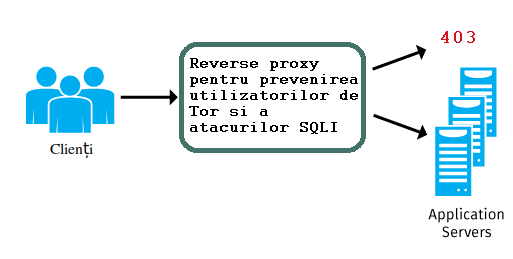
\includegraphics[width=0.6\textwidth]{fff.png}
	\caption{Cutia neagra a sistemului}
	\label{fig:black-box}
\end{figure}

Figura ~\ref{fig:black-box} prezinta cutia neagra a sistemului propus. \\

%\subsection{Functional Specification}
 \subsection{Specificații funcționale}

Sistemul trebui sa prezinte o interfata grafica usor de folosit de catre utilizator si sa fie capabil sa redirectioneze traficul interceptat catre un anumit server, clasificand si filtrand traficul malitios. Pentru a atinge obiectivele proiectului, urmatoarele cerinte functionale trabui indeplinite:
\begin{itemize}
  \item Sa realizere conexiunea la un server HTTP/HTTPS si sa redirectioneze traficul primit catre acesta.
  \item Sa intercepteze traficul venit pe o anumita interfata si port prestabilit.
  \item Sa prelucreze request-urile primite de la clineti intr-un format specific clasificatorului de SQL injection.
  \item Sa nu redirectioneze reqesturile clasificate ca si SQL injection.
  \item Sa blocheze conectarea clientilor ce folosesc ip-uri clasificate ca ip-uri de Tor.
  \item Sa permita utilizatorului sa editez si sa vizualizeze lista ip-urilor de Tor.
  \item Sa prezinte in interfata grafica toate interventiile rezlizate asupra traficului(blocari de conexiuni sau de request-uri).
  \item Sa permita utilizatorului sa configureze modul de operare al sistemului.
\end{itemize}


%\subsection{Non-Functional Specification}
 \subsection{Specificații non-funcționale}

Sistemul trebuie, de asemenea, să aibă următoarele caracteristici non-funcționale pentru a realiza obiectivele specificate:
\begin{itemize}
  \item Sa fie usor de instalat si de folosit pentru orice utilizator, oricat de neexperimentat.
  \item Sa poata intercepta traficul de pe orice/oricate interfete disponibile.
  \item Sa poata rula pe orice sistem de operare Windows cu Python2 instalat.
  \item Sa aiba o rata de blocare de 100\% a ip-urilor de pe lista neagra, iar
  in cazul detectiei de SQL injection sa nu aiba detectii false pozitive mai mari 2-3\%
  si o acuratete generala de peste 90\%
\end{itemize}



